\chapter{Background}
\label{chap:background}


Before we develop the core algorithms and proofs of the thesis, this chapter introduces the fundamentals of \ac{rl}, \ac{mbrl}, and representation learning.
These fields form the basis of the presented research, and the methods and results are built on the established knowledge in these areas.
The definitions and results presented here are well established in the literature and we therefore forgo individual references for each definition.
Instead, readers are referred to appropriate reference work.
The Markov Decision Process is discussed thoroughly in \textcite{puterman1994markov}, and a more general perspective on general continuous state- and action-spaces can be found in \textcite{bertsekasshreve1978}.
For reinforcement learning, thorough introductions are presented in \textcite{suttonbook} and \textcite{farahmand2021}.
The presentation of the Markov Decision Process and Reinforcement Learning basics here roughly follows \textcite{farahmand2011thesis} and \textcite{farahmand2021}.
For model-based reinforcement learning and representation learning, appropriate literature is cited directly as these fields are still in active development.

% This chapter is roughly divided into two halves.
% The first two sections on Markov Decision Processes and Reinforcement Learning provide a textbook style overview of the core concepts used in this thesis.
% Together, they serve the role as a formal introduction and clarification on notation for the topics in this thesis.
% The later sections, while still containing some formalization, serve as condensed surveys of the fields of Model-Based Reinforcement Learning, Representation Learning in Reinforcement Learning, and the idea of Decision Aware Learning.
% These are written with a larger emphasis on the current literature and a formal introduction of relevant ideas are deferred to later chapters in the thesis.


\section{General mathematical notation and definitions}
To define the concepts used in \ac{ml} and especially in \ac{rl} we require some mathematical language.

When talking about sets, we will generally use italic capital letters such as $\states$ or $\actions$, except for canonical notation such as the symbol $\mathbb{R}$ used for the real numbers.
We will use the notational shorthand $\{x\}_N$ and $\{x_1, \dots, x_N\}$ to denote sets containing elements $x_1$ to $x_N$, and $(x_1, \dots, x_N)$ or $(x)_N$ for sequences.

Functions are denoted following standard terminology as lower case letters, and operators use upper case letters.
We will write $M(\mathcal{X})$ to denote the set of possible distributions over the set $\mathcal{X}$ equipped with an appropriate $\sigma$-algebra.
Functions that map to $M(\mathcal{X})$ are called probability kernels and play an important role in the definition of \ac{rl}.
For a probability kernel $\mathcal{P}: \mathcal{X} \rightarrow \mathcal{Y}$ we will use the standard notational shorthand $\mathcal{P}(y|x)$ to denote the probability (density) of $y$ under the distribution $\mathcal{P}$.

Given a suitable probability (density) $p(x)$ for the probability space $(\Omega,\mathcal{F},p)$, we will denote the expectation of a random variable $X: \Omega \rightarrow \mathbb{R}^n$ drawn from $p$ as $\mathbb{E}_{X \sim p}\left[X\right] = \int_{\Omega} X(\omega) \mathrm{d} p(\omega)$.
This makes it clear from what distributions random variables are drawn when several distributions are involved such as in the case of the \ac{kl}.
In a discrete case ($|\states \times \actions| < \infty$), the Lebesgue integral can be simplified to $\sum_{x \in \mathcal{X}} p(x) x$, and in the case of regular real vector valued distributions such as the Gaussian, we will similarly write $\int p(x) x \mathrm{d} x$ and forgo a full measure theoretic treatment.
In these cases we will also not distinguish between random variables $X$ and members of the underlying spaces $x \in \mathcal{X}$ and write $x$ for simplicity.


\section{The Markov Decision Process}
\label{chap:background:mdp}

At the heart of \ac{rl} lies the \textbf{\ac{mdp}} which serves as the core mathematical structure that formalizes the concept of learning in an environment.


\begin{definition}[Markov Decision Process]
An {\ac{mdp}} is a tuple $(\states,\actions,\mathcal{P},r,\gamma)$, where $\states$ is a set of states, $\actions$ is a set of actions, $\mathcal{P}: \states \times \actions \rightarrow M(\states)$ is a transition probability kernel, $r: \states \times \actions \rightarrow \mathbb{R}$ is a reward function, and $\gamma \in [0,1)$ is a discount factor.
\end{definition}

These mathematical objects describe a process in which an agent interacts with an environment over a sequence of discrete time steps.
An agent is said to be in a state $\state \in \states$ at time $t$, where it takes an action $a \in \actions$.
The state at $t=0$ is sampled from a starting state distribution $p_0$.
Note that the state encompasses both the environment and the agent's internal state, such as memory or other information.
There is no strict distinction between internal and external state in the formalism.
The transition kernel is then used to sample a possible next state $\state_{t+1} \in \states$ which the agent transitions to by drawing a sample from $\mathcal{P}(\state'|\state,a)$.
At every timestep, after choosing an action $a$ in state $\state$, the agent receives the reward $r(\state,a)$.
In the case of discrete state-action sets, the next state is drawn from a discrete distributions.
For some results additional care is needed to treat continuous state-action spaces rigorously.
In this thesis, such results are presented in \autoref{chap:cvaml}, where we draw on results from \textcite{bertsekasshreve1978}.
Interested readers are referred there for a more in-depth discussion on continuous state-action spaces.

The word \emph{Markov} in Markov Decision Process refers to the fact that the process is memory-less.
This means that the next state distribution only depends on the current state and action, not on the past history of states.
An agent acting in a \emph{Markov} decision process therefore does not need to remember what happened in the past, all information is captured in the present state.

The agent's strategy for choosing actions is described by its policy, which describes the likelihood of the agent choosing different actions in state $\state$.

\begin{definition}[Policy]
    A policy $\pi: \states \rightarrow M(\actions)$ is a function that maps from states to distributions over actions.
    Given an MDP $(\states,\actions,\mathcal{P},r,\gamma)$ and a policy $\pi$, we denote the \emph{policy-conditioned transition kernel} as $$\mathcal{P}^\pi(\state'|\state) = \int_\actions \pi(a|\state) \mathcal{P}(\state'|\state, a) \mathrm{d} a.$$
\end{definition}

Equipped with definitions for all standard components of the \ac{mdp} and policies, we can now define trajectories and value functions.

\begin{definition}[Trajectories]
    Let $M = (\states,\actions,\mathcal{P},r,\gamma)$ be an \ac{mdp}  .
    We call a sequence of states and actions $\tau^n := (\state_0,a_0,\dots,\state_{n-1},a_{n-1})$ a trajectory of length $n$.
    When $n$ is omitted, we will assume a trajectory of infinite length.
    The likelihood of a trajectory that is generated by an agent following $\pi$ in $M$ is defined as $$p_{M, \pi}(\tau^n) = p_0(\state_0) \pi(a_0|\state_0) \prod_{i=1}^{n-1} \pi(a_i|\state_i) \mathcal{P}(\state_i|\state_{i-1},a_{i-1}).$$
    When the starting state is fixed, we will write $\tau^n_\state$ to signify that all probabilities are condition on $\state$. 
    The probability density is then defined as $$p_{M,\pi}(\tau^n_{\state_0}|\state_0) = \pi(a_0|\state_0) \prod_{i=1}^{n-1} \pi(a_i|\state_i) \mathcal{P}(\state_i|\state_{i-1},a_{i-1}).$$
    In an analogous manner, we can also fix the starting state-action pair to obtain $\tau^n_{(\state,a)}$.
    % We use $\mathcal{T}^n$ to denote the set of all possible trajectories of length $n$ in $M$.
    We denote the sum of discounted rewards associated with a trajectory as $J_\gamma(\tau) = \sum_{i=0}^{n-1} \gamma^i r(\state_i,a_i)$.
\end{definition}

In cases where we are dealing with both timestep indices and sample indices, we will write $\state^{(t)}_i$ where $t$ is the timestep and $i$ is the sample index.
Often, the choice of \ac{mdp}  and policy is clear from context and we will omit the subscripts $\pi,\P$ and $\gamma$ from the notation to avoid clutter.

Trajectories allow us to easily define the value function of a policy.

\begin{definition}[Value function]
    Let $\mathcal{M} = (\states,\actions,\mathcal{P},r,\gamma)$ be an \ac{mdp}  .
    The policy value function $V^\pi: \states \rightarrow \mathbb{R}$ is equal to the expected discounted reward of infinite-length trajectories generated by an agent following policy $\pi$ in $\mathcal{M}$, $$V^\pi(\state) = \mathbb{E}_{\tau_\state \sim p_{\mathcal{M},\pi}(\cdot|s)} \left[ J_\gamma(\tau_\state)\right].$$
    The policy state-action value function $Q^\pi: \states \times \actions \rightarrow \mathbb{R}$ is defined as $$Q^\pi(\state,a) = \mathbb{E}_{\tau_{(\state,a)} \sim p_{\mathcal{M},\pi}(\cdot|\state,a)} \left[ J_\gamma(\tau_{(\state,a)})\right].$$
\end{definition}

This definition has an important caveat -- it assumes that the expectation exists and is finite.
If $\sum_{i=1}^n \gamma^i r_i$ does not converge as $n \rightarrow \infty$, for example because there exists a timestep $t$ so that $r(\state_i,a_i)/\gamma^i \geq 1$ for all $i \geq t$.
To ensure this does not cause issues, we will generally assume that the reward is bounded so that for all state and action pairs $r_{\min} \leq r(\state,a) \leq r_{\max}$.
In this case the value will always be bounded between $(1 - \gamma)^{-1} r_\mathrm{min}$ and $(1 - \gamma)^{-1} r_\mathrm{max}$.
However, there are canonical problems such as the LQR problem for which this does not hold.
In these problems some policies do not induce a (finite) value function.

The goal of the agent in the standard \ac{mdp} framework is to find an optimal policy $\pi^*(\cdot|\state)$ from a set of possible policies $\Pi$ which maximizes the future discounted reward when starting from state $\state$.
Finding such a policy is one of the core goals of \emph{reinforcement learning}, which we discuss in \autoref{chap:background:rl}.

\subsection{Occupancy distributions}

It is often important to characterize the states visited under a policy without considering their temporal ordering.
Sometimes we only care about how likely a state is to appear in any trajectory, not when it appears.
We can formalize this notion by looking at $n$-step transition probabilities.
These are marginals of the trajectory probabilities.

\begin{definition}[N-step Transitions]
    Let $\mathcal{M}$ be an \ac{mdp}   and $\pi$ be a policy.
    The $1$-step probability density $p^1_{\mathcal{M}, \pi}(\state,a|\state_0)$ is defined as $$p^1_{\mathcal{M}, \pi}(\state,a|\state_0,a_0) = \int_\actions \pi(a|\state) \P(\state|\state_0,a_0) \mathrm{d} \pi(a_0|\state_0).$$ 
    The $n$-step transition is defined recursively as $$p^n_{\mathcal{M}, \pi}(\state,a|\state_0) = \int_{\states,\actions} \pi(s|a) \P(\state|\state_{n-1},a_{n-1}) \mathrm{d} p^{n-1}_{\mathcal{M}, \pi}(\state_{n-1},a_{n-1}|\state_0) .$$
    Analogous to the trajectory case, $p^n_{\mathcal{M}, \pi}(\state,a|\state_0,a_0)$ is the n-step probability resulting from the state-action pair $(\state_0,a_0)$.
\end{definition}

Summing up and discounting $n$-step transitions results in the discounted state-action occupancy measure.

\begin{definition}[Discounted state-occupancy measure]
    Let $\mathcal{M}$ be an \ac{mdp} and $\pi$ be a policy.
    The discounted state occupancy distribution $\rho_{\mathcal{M},\pi}(\state,a|\state_0,a_0)$ is the distribution constructed as $$\rho_{\mathcal{M},\pi}(\state,a|\state_0,a_0) = \frac{1}{1 - \gamma} \sum_{i=0}^\infty \gamma^i p^i_{\mathcal{M},\pi}(\state,a|\state_0,a_0).$$
\end{definition}

Finally, in the case of \emph{positive recurrent} transition kernels the sequence $p^n_{M,\pi}$ converges in distribution for $n \rightarrow \infty$.
If this distribution is independent of the start state-action pair (which requires a positive recurrent and aperiodic transition kernel), we call it the stationary state-action distribution and write $\mu_{M,\pi}(\state,a)$.

\subsection{State and action observations}

In the most general formulation of the \ac{mdp}   presented here, we do not place additional assumptions on the structure and relationships between the states and actions in $\states$ and $\actions$.
In practice, however, such structure exists for many interesting problems and can be exploited for learning.
One important way in which structure is captured in practice is through state and an actions \emph{observations}, which are crucial for the success of an \ac{rl} algorithm.
The observation of the state and action space can be seen as a mapping from the abstract state space to a concrete observation space, such as a vector of real numbers or an image.

A state observation function maps each state $\state\in\states$ into an observation space $\mathcal{Y}$, often one that is equipped with structure such as $\mathbb{R}^n$.
Most of the time we will not distinguish between a state (or action) and its observation.
However, when we need to explicitly talk about such a function, we will denote it as $o: \states \rightarrow \mathcal{Y}$.
Common hand-crafted observation functions map discrete states to one-hot vectors, or follow more complex schemes such as tiling activations.

If the state observation function is not invertible, the resulting problem is called a \ac{pomdp}.
In this framework, an agent cannot discern from the observation alone in which state it currently is, and needs to use other information, such as the past history of observations.
In general, this thesis will stick to the realm of fully observable MDPs and steer clear of \acp{pomdp}.
Nonetheless, they are an important class of problems in their own right, especially for modelling real world phenomena in which full observability is rarely, if ever, given.

It is not uncommon for an \ac{mdp} problem to have more than one way to represent states via observations.
For example, in many robotic control tasks, the state can either be represented as a set of joint angles and velocities, or by a sequence of camera images from the robot, or even a combination thereof!
Often, changing the observation space can make a problem much harder or simpler to learn in practice.

One simple example of this is the representation of angles, a common problem in many real-world applications such as robotics.
An angle $\theta$ can be represented as a numerical value $\theta \in [0,2\pi)$.
However, this representations has a discontinuity from $2\pi$ to $0$.
For example, adding a small angle $\delta\theta$ to $\theta$ will generally result in a new angle $(\theta + \delta\theta)~\mathrm{mod}~2\pi$.
If the same angle is instead represented as the vector $[\sin(\theta),\cos(\theta)]$, addition does not result in a discontinuous functions.
However, this has the drawback that not all two dimensional vectors denote valid angles, and angular addition is not a linear operation.

The problem of mapping from a state or its observation to a space that is beneficial for the goal of learning a good policy is called \emph{representation learning}, and will be a major focus of this thesis.
In general, we will assume that \emph{observations} are mappings that are inherent to the problem and unchangeable from the perspective of the algorithm, while \emph{representations} are mappings that the agent can change.
However, this distinction is not always cleanly followed in the literature and observations are sometimes also referred to as representations.


\section{Reinforcement Learning}
\label{chap:background:rl}

Now that the problem of finding an optimal policy is established, we need algorithms to solve it.
In this section, we review the basic concepts of \ac{rl} that are used to obtain optimal policies.
Given the scope of this thesis, we will focus solely on value driven methods that learn value functions and use these to improve upon the policy.

\subsection{Reinforcement Learning in Tabular Domains}

When the state and action sets are finite, all relevant components of the \ac{mdp} problem can be represented by vectors and matrices.
If the MDP has $n = |X|$ distinct states, the policy-conditioned transition kernel $\P^\pi$ becomes a matrix of shape $n \times n$, and the reward and state value function a vector of shape $n$.

Following standard Markov chain notation, any distribution over states is written as a row vector $\mathbf{\state} = [p(\state_1),\dots, p(\state_n)]$ and the transition probability is given as $$\left[\sum_{i=1}^n \P(\state_0|\state_i), \dots, \sum_{i=1}^n \P(\state_n|\state_i)\right] = \mathbf{\state} \P^\pi.$$
The expected reward over a state distribution is also easily expressed as an inner product $\langle \mathbf{\state},r\rangle.$
We will frequently make use of the fact that $V^\pi = \sum_{i=0}^\infty \gamma^i \P^i r = (I - \gamma \P^\pi)^{-1}r$.
This again assumes that the infinite sum converges, as discussed previously.
Beyond the results presented here which are foundational for all chapters, we present some additional results and lemmas, mostly taken from the literature in \autoref{app:formal}.
These are specifically relevant for \autoref{chap:understanding} and \autoref{chap:cvaml}.

\subsection{Bellman optimality and Bellman operators}

When looking at the definition of the policy value function, we can quickly see that it is recursive.
We can decompose the value function into the first step reward and the next state's value $$V^\pi(\state) = \mathbb{E}_{a\sim\pi(\cdot|\state)}\left[r(\state,a) + \gamma \mathbb{E}_{\state'\sim\P(\cdot|\state,a)}\left[V^\pi\left(\state'\right)\right]\right].$$

This decompositions allows us to use one of the central concepts of reinforcement learning and dynamic programming: the Bellman Optimality Principle:
\begin{quote}
    An optimal policy has the property that whatever the initial state and initial decisions are, the remaining decisions must constitute an optimal policy with regard to the state resulting from the first decisions. \parencite{bellman1953}
\end{quote}
Assuming that an agent will follow the current policy in the subsequent state, an agent can improve its policy based on the current value function by computing $$\pi_\mathrm{new}(\state) = \argmax_{a \in \actions} \left[r(\state,a) + \gamma \mathbb{E}_{\state'\sim\mathcal{P}(\cdot|\state,a)}\left[V^\pi\left(\state'\right)\right]\right].$$

The corresponding value function then becomes
$$V^{\pi_\mathrm{new}}(\state) = \max_a \left[r(\state,a) + \gamma \mathbb{E}_{\state'\sim\mathcal{P}(\cdot|\state,a)}\left[V^\pi\left(\state'\right)\right]\right] \geq V^\pi(\state).$$

By greedily picking the best action under the one step reward and the \emph{current} policy's value function, the agent is guaranteed to receive at least the same future reward in each state as previously.
This lays the foundation for a whole class of methods that all follow the same recipe: pick a policy, compute its value function, improve the policy based on the value function, and repeat.
The standard examples of such algorithms are \ac{pi} and \ac{vi}, which require full knowledge of the transition kernel and reward.

\paragraph{Policy Iteration}

In policy iteration, we begin by fixing a policy and computing its value function.
Doing this takes advantage of the recursive nature of the function by the way of a fixed point iteration.
Given any appropriate function $Q: \states \times \actions \rightarrow \mathbb{R}$, we can define the Bellman operator as follows.

\begin{definition}[On-policy Bellman Operator]
    Let $\mathcal{M}$ be an MDP, $\pi$ be a policy, and $Q: \states \times \actions \rightarrow \mathbb{R}$ any function mapping state-action pairs to real numbers.
    The Bellman Operator $\mathcal{T}^\pi$ is defined as
    $$[\mathcal{T}^\pi Q](\state,a) = r(\state,a) + \gamma \mathbb{E}_{\state'\sim \mathcal{P}(\cdot|\state,a)}\left[\mathbb{E}_{a'\sim\pi(\state')}\left[Q(\state',a')\right]\right]$$ for all states and actions in the MDP.
\end{definition}

The true policy state-action value function $Q^\pi$ is the fixed point of this operator $[\mathcal{T}^\pi Q^\pi] = Q^\pi$.
When starting with any initial function $Q$, repeatedly applying the Bellman Operator converges results in a fixed-point iteration that can be proven to converge to $Q^\pi$ using Banach's Fixed Point Theorem.

With this $Q$ function, we can define our new policy as $\pi^\mathrm{new}(\state) \leftarrow \argmax_{a\in\actions} Q(\state,a)$ and then repeat the process.
This can be proven to converge to the optimal policy $\pi^*$, by noticing that we have guaranteed improvement in $\pi$ and that the process cannot get stuck in a local optimum.
For a full proof, refer to \textcite{farahmand2021}.

\paragraph{Value Iteration}

Instead of waiting for our Bellman iteration to complete for each policy, we can instead greedily update the policy at every step.
This leads to the so called Bellman optimality operator.

\begin{definition}[Bellman Optimality Operator]
    Let $\mathcal{M}$ be an MDP, $\pi$ be a policy, and $V: \states \rightarrow \mathbb{R}$ any function mapping state-action pairs to real numbers.
    The Bellman Optimality Operator $\mathcal{T}^*$ is defined as
    $$[\mathcal{T}^* Q](\state,a) = r(\state,a) + \gamma \mathbb{E}_{\state'\sim \mathcal{P}(\cdot|\state,a)}\left[\max_{a' \in \actions}Q(\state',a')\right].$$
\end{definition}

This again can be shown to converge directly to the $Q$ function of the optimal policy.

\subsection{Parametric value function learning}

As the state-action space of an \ac{mdp} grows larger, keeping an explicit record of each state's value in a long vector becomes less and less feasible.
Memory requirements grow linearly with the size of the state-action space.
In addition, we are not able to make use of additional structure in the state-spaces, such as meaningful observation functions.
Therefore, it is generally useful to leverage approximations which are efficient to store and can make use of structure.
In this thesis, we are foremost interested in parametric approximations.

\begin{definition}[Parametric approximation]
    A parametric approximation of a value function is defined by a $k$-dimensional vector $\omega \in \mathbb{R}^k$ and a function $V: \states \times \mathbb{R}^k \rightarrow \mathbb{R}$.
\end{definition}

In this thesis, we will mostly consider neural networks and use linear function approximations in \autoref{chap:understanding} to develop a theoretical model of representation learning.

Once we have parameterized function, we cannot simply apply the Bellman operators in closed form as we did to obtain \ac{vi} and \ac{pi} in the tabular domain.
To obtain the optimal weights of a parametric value function, we require a learning algorithm.
While there is a huge variety of such algorithms, many currently popular ones revolve around the same core concept, approximate value or policy iteration.
Approximate value iteration seeks a function in each iteration that is as close to $[\mathcal{T}V]$ as possible.
To understand how to achieve this, we will quickly review some core concepts in machine learning and \ac{erm}.

\subsubsection{Empirical Risk Minimization}

In machine learning, the most common way to find the optimal parameters of a function is by minimizing a loss function.
Given a parametric function $f_\theta(x): \states \rightarrow \mathcal{Y}$ from some function class $\mathcal{F}_\theta$, and prediction targets $y$, the loss function $l: \mathcal{Y} \times \mathcal{Y} \rightarrow \mathbb{R}$ is computed to measure the error between the prediction and the target.
Often, these loss functions are distance functions such as the squared $L_2$ distance $l(y, f_\theta(x)) = \|y - f_\theta(x)\|^2.$

The goal of \ac{erm} is minimize the expected loss of our function estimation under some distribution $P$ over data points $x$ and targets $y$.
Formally, we aim to find $$f^* = \argmin_{f_\theta\in\mathcal{F}_\theta} \int l(y, f_\theta(x)) \mathrm{d} P(x,y).$$
However, we generally do not have access to the distribution $\mu$ in a way that allows us to freely sample unlimited data points $(x,y)$.
Therefore, we instead assume access to a fixed dataset $D = \{(x_1, y_1) \dots, (x_N, y_N)\}$ which is distributed according to $P$ and define $\mathcal{L}(f_\theta,D) = \frac{1}{|D|} \sum_{i=1}^N l(y_i, f(x_i))$.
Then the optimal function $f^*$ according to the empirical measure defined via $D$ is $$\hat{f}^* = \argmin_{f_\theta \in \mathcal{F}_\theta} \mathcal{L}(f_\theta,D).$$
We will generally use the notation $\mathbb{E}_D$ interchangeably with $\mathbb{E}_P$ throughout this thesis to signify an expectation taken across every possible dataset taken from $P$.

The study of when and how quickly the empirically optimal function $\hat{f}^*$ approaches the function that minimizes the expected loss over the underlying distribution $f^*$ is an important area of research in machine learning.
In this thesis, we will focus on examples of loss functions which are mis-calibrated, which means that $\hat{f}^*$ does not converge to $f^*$ as we increase the size of the dataset.
In the next section, we will review the well-known case of the double sampling problem, and we will encounter this problem again in \autoref{chap:cvaml} in the context of decision-aware model losses.
We will also introduce the notion of mis-calibration formally there.

\subsubsection{Loss functions for Value Learning}
The value function $V^\pi$ could in principle be obtained from trajectories of the current policy, by computing $$\mathcal{L}(\hat{V}, \{\state, \tau_{\state}\}_N) = \frac{1}{N} \sum_{i=1}^N \left(J(\tau_{\state_i}) - \hat{V}(\state_i)\right)^2.$$
Such an approach is called a Monte Carlo approach, as it relies on a Monte Carlo or sample-based approximation of the value function.
However, the Monte Carlo approach does not take advantage of the Bellman decomposition of the value function.

If we use this structure, we can greatly improve the sample efficiency of our approach, as we do not need to collect full trajectories for each state we want to estimate the value function on.
To do this, we need to define a loss function that depends on the value estimate in the target as well.

\paragraph{Bellman Residual Minimization and the Double Sampling Problem}
Naively, we might want to try and minimize a loss function of the form
$$\mathcal{L}_\mathrm{res}\left(\hat{V}, \{\state, r, \state'\}_{N}\right) = \frac{1}{N} \sum_{i=1}^N \left(\hat{V}(\state_i) - r_n - \gamma \hat{V}(\state'_i)\right)^2.$$
This is called \emph{Bellman Residual Minimization}, and we can show that it does not lead to a correct value function estimate.
This result is well known in the reinforcement learning literature, see e.g. \textcite[p. 299]{suttonbook}.
We will briefly review the proof here as similar techniques will be relevant to show issues with similar loss functions in \autoref{chap:cvaml}.


\begin{proposition}[The Double Sampling Problem]
    Let $D$ be a dataset of $(\state_i,r_i,\state'_i)$ tuples sampled from the stationary distribution of some \ac{mdp}  $\mathcal{M}$ with transition kernel $\P$ and fixed policy $\pi$.
    There exist function classes $\mathcal{V}$ that include $V^\pi$, the ground truth value function for $\P^\pi$, but for which 
    \[V^\pi \notin \argmin_{\hat{V} \in \mathcal{V}} \mathbb{E}_{x,r,x' \sim \mu} \left[\mathcal{L}_\mathrm{res}(\hat{V}, \{\state, r, \state'\})\right].\]
\end{proposition}

The proof is relatively straight forward.
We need to show that the intended target, $V^\pi$, does not properly minimize the loss.
To do this, we decompose the loss function as follows
\begin{align}
    \mathbb{E}_{\mu} \left[\mathcal{L}_\mathrm{res}(\hat{V}, \{\state, r, \state'\}_N)\right] &= \mathbb{E}_{D} \left[\frac{1}{N} \sum_{n=1}^N \left(\hat{V}(\state_n) - r_n - \gamma \hat{V}(\state'_n)\right)^2\right] \\
    &=\mathbb{E}_{\mu} \left[\left(\hat{V}(x) - r - \gamma \hat{V}(x')\right)^2\right] \\
    &=\mathbb{E}_{\mu} \left[\left(\hat{V}(x) - V^\pi(x) + V^\pi(x) - r - \gamma \hat{V}(x')\right)^2\right] \\
    &=\mathbb{E}_{\mu} \left[\left(\hat{V}(x) - V^\pi(x)\right)^2\right] + \mathbb{E}_{D}\left[\left( V^\pi(x) - r - \gamma \hat{V}(x')\right)^2\right] \\
    &\quad + 2 \mathbb{E}_{\mu}\left[\left(\hat{V}(x) - V^\pi(x)\right)\left( V^\pi(x) - r - \gamma \hat{V}(x')\right)\right]
\end{align}

If we substitute the true value function $V^\pi$ for $\hat{V}$, it is easy to see that the first and last terms disappear.
However, we are left with a variance like term
\begin{align}
    \mathbb{E}_{D} \left[\mathcal{L}_\mathrm{res}(V^\pi, \{x, r, x'\}_N)\right] &= \mathbb{E}_{D} \left[\frac{1}{N} \sum_{n=1}^N \left(V^\pi(x_n) - r_n - \gamma V^\pi(x'_n)\right)^2\right] \\
    &=\mathbb{E}_{D} \left[\left(\underbrace{V^\pi(x) - V^\pi(x)}_{=0}\right)^2\right] + \mathbb{E}_{D}\left[\left( V^\pi(x) - r - \gamma V^\pi(x')\right)^2\right] \\
    &\quad - \mathbb{E}_{D}\left[\underbrace{\left(\hat{V}(x) - V^\pi(x)\right)}_{=0}\left( V^\pi(x) - r - \gamma \hat{V}(x')\right)\right]\\
    &=\mathbb{E}_{D}\left[\left( V^\pi(x) - r - \gamma V^\pi(x')\right)^2\right] > 0.
\end{align}

Our formal statement requires a function that minimizes this loss better than the ground truth value function in our function class.
We will discuss the existence of such functions and provide examples in \autoref{chap:cvaml}.

If we had two independent next state samples $x'_i$, we could construct an unbiased estimator of the target and obtain a correct loss.
But in the standard \ac{rl} setting, we assume strict sequential interaction.
So in general we cannot rely on having two independent samples for each state whose value we want to estimate.

\paragraph{Target Network Updates}

Instead of naively minimizing the predicted difference between our current value function estimate, we only need a minimal change to make the loss function work.
We cannot update the parameters of both the value estimate $\hat{V}$ and the bootstrapped Bellman estimate $R + \gamma \mathcal{P}^\pi \hat{V}$.
So instead, we make use of an independent copy of the value function, $\hat{V}_\mathrm{target}$, which is commonly called a target network. 
This target network is periodically updated towards the current value estimate $\hat{V}$.
With the help of the target network, we can define
\[
    \mathcal{L}_\mathrm{TD}\left(\hat{V}, \hat{V}_\mathrm{target}, \{x_i, r_i, x'_i\}_{n}\right) = \frac{1}{n} \sum_{i=1}^n \left(\hat{V}(x_i) - \left[r + \gamma \hat{V}_\mathrm{target}(x'_i)\right]_\mathrm{sg}\right)^2
\]
as our loss.
The notation $[\cdot]_\mathrm{sg}$ refers to a \emph{stop gradient} operation, which clarifies that the loss function is not used to update the later part of the equation.

Different algorithms choose different approaches to obtain the target estimate $\hat{V}_\mathrm{target}$.
The simplest two variants are to either replace $\hat{V}_\mathrm{target}$ at \emph{every} update step, or instead to wait until $\hat{V}$ has converged to an optimum and update then.
The later mimics the structure of the Bellman fixed-point iteration, but as it can take a lot of iterations for the value estimate to converge fully, this can be computationally expensive.
On the other hand, updating the target at every step can prove to be very unstable in practice.
Instead of these extremes, most common algorithms either use a fixed, but large, update period, e.g. 1000 steps, \parencite{dqn} or use a Polyak average of the parameters $\theta_\mathrm{target} \leftarrow (1 - \alpha) \theta_\mathrm{target} + \alpha \theta$ with a small value for $\alpha$ \parencite{td3}.

The introduction of a bootstrapped target that depends on the value estimate itself lies at the heart of (almost) all problems discussed in this thesis.
With this design choice, we have introduced non-stationarity in the targets of our optimization problems which leads to unstable optimization.
However, it is crucial to understand that we do not make this decision lightly.
Relying on the Bellman backup instead of Monte-Carlo estimates makes many of our algorithms vastly more efficient.
As our goals are stable \emph{and efficient} value learning, we will therefore not avoid but embrace the use of bootstrapped target estimation.

\paragraph{Policy improvement}

After establishing a loss function that can be used to learn parametric value function approximations, we can apply (approximate) \ac{vi} or \ac{pi} to obtain policy updates.
As in the tabular case, we can interleave policy update steps with value function approximation steps, or extract a policy from a fully converged value function.
However, the former is used by almost all modern \ac{drl} algorithms, as waiting for the value function to converge can take a long time.

When the action space is tabular, a policy can be obtained from an approximate Q function by choosing $a \in \argmax_{\mathcal{A}} Q(\state,a)$.
However, when the action space is continuous, we also have to parametrize the policy.
In this thesis, we will mostly rely on the \ac{dpg}, which is introduced in \autoref{sec:background:drl}.

\paragraph{On- and off-policy learning}

In addition to a loss function, we also need a dataset to train on.
Here, two major strategies dominate: on-policy and off-policy learning.

In \emph{on-policy} learning, all data comes from a single policy, the one for which we are attempting to estimate the value.
While this is generally much more stable, it also requires a large amount of samples, as we need to gather new data from scratch once we change the policy.
In principle, old samples can be used if we apply a sampling correction term such as importance sampling.
But even in this case, the importance weights quickly become too small for old samples to have an impact on the loss.
As this thesis is interested in \emph{efficient} learning, we instead focus on off-policy learning.

In \emph{Off-policy} learning we reuse samples from old policies, which makes the approach more sample-efficient, but introduces several algorithmic challenges.
% Firstly, we are forced to rely on state-action value functions (Q) instead of state value functions (V), as we cannot improve our policy otherwise.
Many algorithms can diverge when used with off-policy samples, even when their on-policy counterparts converge.
The combination of bootstrapped value estimation, function approximation, and off-policy learning has therefore been termed as the \emph{deadly triad} by \textcite{suttonbook}.
Nonetheless, all components of the deadly triad are useful or sometimes even necessary (in the case of function approximation) to scale \ac{rl} to complex problems.
While most chapters in this thesis deal with problems resulting from the deadly triad in one form or another, we will focus on off-policy learning specifically in \autoref{chap:mad}.

\subsection{Deep Reinforcement Learning in Continuous Action Spaces}
\label{sec:background:drl}


Current \ac{drl} methods use several additional mechanisms to ensure stable training of the \ac{rl} agent's value function and policy with neural networks.
Here, we take a brief look at the \ac{td3} \parencite{td3} and \ac{sac} \parencite{sac} algorithms, as they are used throughout the empirical work presented in this thesis.

Both \ac{td3} and \ac{sac} are actor-critic algorithms, which interleave value function and policy updates.
They are built for continuous state-action spaces and estimate state-action value functions.
In addition, they use parameterized policies, as the policy update cannot be solved in closed form.
Actor-critic algorithms therefore replace the closed form maximization with another gradient based update.
In the case of \ac{td3} and \ac{sac}, this is the \ac{dpg} \parencite{silver2014deterministic} which uses the fact that neural network based Q approximations are differentiable with regard to their inputs
\begin{align}
    \theta_\pi \leftarrow \theta_\pi + \alpha \nabla_{\theta_\pi} Q(s, \pi(\state, \theta_\pi)).
\end{align}
While \ac{td3} uses a deterministic policy $\pi: \states \rightarrow \actions$, \ac{sac} uses a probabilistic Gaussian policy and computes the gradient using the re-parameterization trick
\begin{align}
    \nabla_{\theta} \EEX{y \sim \mathcal{N}(\mu_\theta(x), \sigma_\theta(x))}{f(y)} \approx \frac{1}{N} \sum_{i=1}^{N} \frac{\mathrm{d}\,f(y)}{\mathrm{d}\, y}\bigg|_{y = \mu_\theta(x) + \epsilon_i \sigma_\theta(x)}  \frac{\mathrm{d}\,y}{\mathrm{d}\,\theta}\bigg|_{y = \mu_\theta(x) + \epsilon_i \sigma_\theta(x)},
\end{align}
where each $\epsilon_i$ is sampled independently from $\mathcal{N}(0,1)$.

The main innovation of \ac{td3} is the introduction of the twinned critic to counterbalance overestimation in the critic estimation.
The overestimation problem stems from the fact that the actor is updated to maximize the critic's prediction.
If the critic estimate is noisy, the selected action's value will in general be larger than the true value.
Due to this, the Bellman operator will propagate this overestimation into the Q function, which will inflate the Q values over time.

To counterbalance this, \textcite{fujimoto2018addressing} introduce two independent critic estimates $Q_1$ and $Q_2$.
The double critic's loss function is
\begin{align}
    \mathcal{L}(Q_i| \state, a, r, \state', \pi) = \left(Q_i(\state,a) - \left[r + \gamma \min_{j \in [1,2]}Q_j(\state', \pi(\state'))\right]\right)^2.
\end{align}
The actor update also maximizes this minimum over both critics
\begin{align}
    \mathcal{L}(\pi| \state, Q_1, Q_2) = - \min_{j \in \{1,2\}} Q_i(\state, \pi(\state)).
\end{align}
With some assumptions on the noise this max-min structure can be proven to prevent overestimation.
However, as will be discussed in \autoref{chap:overestimation}, these assumptions are not met in practice.
Therefore, while this trick is helpful, by itself it is insufficient by itself to prevent overestimation.
In addition to statistical error, the optimization process of the critic can be unstable and lead to overestimation.

\ac{sac} uses the double critic structure of \ac{td3} and modifies the critic to optimize a maximum entropy objective.
For this, the critic target is modified to include the stochastic policy's entropy over the next state
\begin{align}
    \mathcal{L}(Q_i| \state, a, r, \state', \pi) = \left(Q_i(\state,a) - \left[r + \gamma \min_{j \in [1,2]}Q_j(\state', a') - \log \pi(a'|\state')\right]\right)^2, \quad a'\sim\pi(\cdot|\state').
\end{align}
The policy objective function is similarly modified
\begin{align}
    \mathcal{L}(\pi| \state, Q_1, Q_2) = - \min_{j \in [1,2]} Q_i(\state, a) + \log \pi(a|\state), \quad a\sim\pi(\cdot|\state).
\end{align}
This maximum entropy modification can be interpreted in the framework of ``control-as-inference'' \parencite{levine2018reinforcement} and has been shown to be empirically more stable than \ac{td3}.
However, it is also computationally slightly more expensive as it involves a sampling operation, and so several algorithms proposed in this thesis will use \ac{td3} instead of \ac{sac}.
Our insights are generalizable to most algorithms from the \ac{dpg}/\ac{td3}/\ac{sac} family.

\section{Model-Based Reinforcement Learning}
\label{sec:model_learning}

Many reinforcement learning algorithms compute their value functions and policies directly based on past data from the environment.
In \ac{mbrl} on the other hand, a predictive \emph{model}\footnote{\emph{Model} is a notoriously ambiguous term in machine learning. In the context of this thesis, the word \emph{model} is used solely to describe an approximation of a transition function, reward function, or a similar object, while neural networks and other types of function approximators will be referred to as \emph{function approximators} or simply \emph{functions}.} of the environment is trained and used in the \ac{rl} algorithm.
This model can be used to augment the learning, either by providing additional data as in the Dyna architecture \parencite{dyna}, or by providing gradient estimates \parencite{hafner2020dream,amos2021model}, or simply to enhance the representation learning as we will discuss in \autoref{chap:understanding}.

The most common kind of model used in \ac{mbrl} is a \emph{forward prediction model}.
This is a parameterized function, such as a neural network, that takes a state-action pair as an input and predicts the next state.
Simple extensions to these include multi-step models which use sequences of actions to predict short-horizon trajectories and stochastic models which parameterize distributions over next states.

\begin{definition}[Types of environment models]
    A probabilistic \emph{forward prediction model} is a parameterized distribution $\hat{p}_\theta(x'|x,a)$ that approximates an \ac{mdp}'s transition kernel.
    
    A \emph{deterministic} forward prediction model is a function $f: \states \times \actions \rightarrow \states$ that directly maps to a next state.

    A deterministic \emph{latent} forward prediction model is a combination of an embedding function $\phi: \states \rightarrow \mathcal{Z}$ that maps from the state space $\states$ to a latent space $\mathcal{Z}$, and a latent dynamics model $f_\mathcal{Z}: \mathcal{Z} \times \actions \rightarrow \mathcal{Z}$.
    Unless specified otherwise, we assume that $\mathcal{Z} = \mathbb{R}^k$, where $k$ is the dimensionality of the latent space.
    Trajectories from a latent model are sampled conditioned on the embedding of an initial state $x_0$.
\end{definition}

All relevant definitions from \autoref{chap:background:mdp} can be extended for environment models and we will generally use the notation $\hat{p}$ or $\hat{f}$ to differentiate a learned environment model from the ground truth.

Probabilistic latent environment models are also possible and are defined as one would expect via kernels over next latent states.
We will revisit probabilistic latent dynamics models in the context of decision-aware learning in \autoref{chap:cvaml}.
There are several other types of models, such as inverse dynamics models which seek to predict actions given a state and its successor, but in this thesis, we will focus on the more common forward predictive models.

\subsection{Training the model}

Most commonly, models are trained by obtaining a dataset $\mathcal{D}$ of transition tuples consisting of states $x$, actions $a$, reward $r$, and next states $x'$. 
Often these datasets are obtained online during interaction with the environment, but they can also come from other offline sources such as human demonstrations.

Given a dataset, an approximate model $\hat{p}$ can be trained using a \ac{mle} objective 
\begin{align}
\max_{\hat{p}} \frac{1}{N}\sum_{i=1}^N \log \hat{p}(x_i'|x_i,a_i).
\end{align}
For example, a Gaussian environment model, such as the ones used by \textcite{pets,janner2019mbpo} as well as in \autoref{chap:vagram}, uses the Gaussian negative log likelihood over a dataset as the loss function
\begin{align}
    &\mathcal{L}_\mathrm{model}(\mu_\theta, \Sigma_\theta; D) = - \frac{1}{N} \sum_{i=1}^N \left[\log \mathcal{N}(x_i' | \mu_\theta(x_i,a_i), \Sigma_\theta(x_i, a_i)) \right].
\end{align}
For deterministic models, a common objective is the \ac{mse}
\begin{align}
    &\mathcal{L}_\mathrm{model}(f_\theta; D) = \frac{1}{N} \sum_{i=1}^N (x'_i - f_\theta(x_i, a_i))^2.
\end{align}

These methods are commonly referred to as \emph{reconstruction objectives} or \emph{observation prediction} objectives (compare \autoref{chap:understanding} for a thorough discussion), as the learned model predicts $x'$ as it is provided by the environment or dataset.
Later in this thesis, we will discuss \emph{latent space models} more thoroughly as an alternative.

In addition to the next state, environment models are often trained to predict the reward as well, as the reward function is not generally assumed to be known.
To do this, the model's output is extended by an additional scalar $\hat{r}_\theta(\state)$ and we add $|r(\state) - \hat{r}_\theta(\state)|^2$ to the loss function.
Unless noted otherwise, we will generally assume that the reward function is predicted using the model whenever the model is used.

\subsection{Using the model}

Of course learning a model is not sufficient on its own.
If our ultimate goal is better agents, we also have to use the model in our \ac{rl} algorithms.
Here, we will very briefly survey common ways of using the model to improve different aspects of \ac{rl} algorithms, which are also used in this thesis.
However, many more ways of using a model have been proposed in the literature, and so interested readers are referred to the survey presented by \textcite{moerland}. 

\subsubsection{Dyna}

\begin{figure}
    \centering
    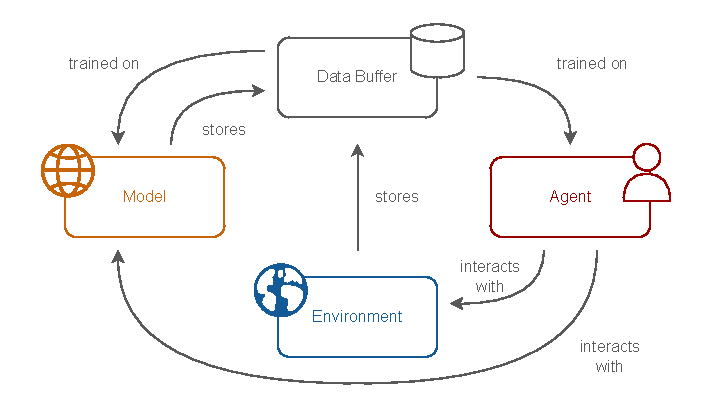
\includegraphics[width=.8\textwidth]{illustrations/thesis_background_dyna.pdf}
    \caption{A sketch of the Dyna framework. The RL agent collects data from the real environment and stores this in a replay buffer. This replay buffer is used to train a model of the environment, which acts as a copy of the environment from the perspective of the agent. Algorithms differ in the question how long model generated data is stored in the replay buffer. While \textcite{janner2019mbpo} for example keeps model generated data for a few thousand update steps, the model-based algorithms presented in \autoref{chap:cvaml} and \autoref{chap:mad} do not store the data for multiple steps at all and generate it anew for each agent update.}
    \label{fig:background:dyna}
\end{figure}


The Dyna framework \parencite{dyna} is one of the most common ways of using an environment model in \ac{rl}.
The main idea is very simple: instead of only using the real environment for generating transition samples $\{x,a,r,x'\}$ we use the model as well.
The concept is sketched out in \autoref{fig:background:dyna}.
In this setup, the use of the model is mostly invisible to the \ac{rl} algorithm which computes the value function and policy.
This makes it very flexible, as we can freely vary the model training and \ac{rl} algorithm without changing the overall framework.

There are several advantages to using the model in addition to the environment.
The simplest is that we are able to generate synthetic data in addition to data from the real environment.
If this data is similar enough to real data, this allows us to increase the sample efficiency of the \ac{rl} training, by simply generating additional data.
Whether this leads to strong performance improvements in applications however depends on how accurate we can make the model with limited data.
If we need as many samples to obtain an accurate model as we need to learn a good value function or policy, the performance gains from Dyna might be limited.

An additional advantage of Dyna is that the model can serve as an oracle simulator.
This means that we can get a next state $\state'$ for any $\state,a$ pair we query the model on.
In the real environment we are instead forced into a sequential interaction where we cannot freely choose the input state $\state$.
\ac{rl} with an oracle generative model can be shown to be optimal in a minimax sense \parencite{agarwal2020model}.
However, the theoretical results rely on obtaining a maximum likelihood model with a well-specified model class.
In practice, we are often not able to learn a sufficiently correct oracle model, and so again, gains in efficiency have to be weighed against model errors influencing the learned value and policy.
We will discuss the impact of model errors on learning extensively in the next section.

As the Dyna framework is relatively flexible, many works in the literature propose algorithms which build on the general idea of learning a model and generating samples from it.
We will review Dyna more closely in \autoref{chap:vagram} and discuss related work.
In \autoref{chap:mad}, we will discuss how using Dyna and specifically the ability to query the model freely with visited states and on-policy actions can greatly stabilize value function learning.

\subsubsection{Online Planning}

While the Dyna framework focuses on improving the value and policies of the agent from stored experiences, a model can also be used to improve the policy as it is being executed.
Depending on the structure of the MDP, proposed methods include random shooting \parencite{pets}, \ac{mcts} \parencite{silver2016mastering,schrittwieser2020mastering}, or \ac{mpc} \parencite{hansen2022temporal,hansen2024tdmpc}.
While the details of the techniques vary, they all follow a similar base formula.

Starting from the current state $\state$ that the agent is in, the agent uses a search policy to query the world model for possible future trajectories.
In the simplest case, random shooting, the agent simply collects $n$ trajectories from the world model by adding random noise to its current policy, or drawing samples from a stochastic policy, and computes the Monte-Carlo estimate of the expected return with regard to the model.
It then executes the most promising action according to these return estimates.
\ac{mcts} and \ac{mpc} can be seen as refinements of this simple techniques where the search procedure is refined by selectively searching over promising future states in the case of \ac{mcts}, or refining the initial action samples iteratively in the case of \ac{mpc}.

In this thesis we will use \ac{mpc}-based methods in \autoref{chap:mad} to improve upon a base policy using a learned model.

\subsubsection{Other ways to use a model}

Beyond learning with Dyna and planning, models can be incorporated into learning in a variety of other ways.
Again, while a thorough survey of model-based reinforcement learning is out of scope for this thesis, we will highlight some additional ideas here as they are relevant for this thesis and related work.

\paragraph{Model-based representation learning:} Instead of using the model directly as an oracle or simulator, a model learning loss can be used to improve the intermediate representations of a neural network-based agent.
This technique is one example of learning with \emph{auxiliary} tasks \parencite{jaderberg2017reinforcement}.
This idea will become an important aspect of this thesis, and will be the focus of \autoref{chap:understanding}.
Therefore we forgo a lengthy introduction here and refer readers to the upcoming chapter.

\paragraph{Differentiating a learned model:} As neural networks have become the de-facto standard way to obtain an environment model in the current machine learning literature, we automatically obtain an additional useful characteristic from this choice: gradients.
As most neural networks are end-to-end differentiable with regard to both their parameters and their inputs, we can use this fact to directly differentiate the model-based return estimate with regard to an action sequence or policy to improve learned policies by differentiating straight through a multi-step bootstrapped rollout.
This technique is succinctly described in \textcite{amos2021model} and used in works such as \textcite{hafner2020dream}.
\textcite{voelcker2022value} discusses differentiable models in the context of decision-aware learning.

\subsection{Abstract latent value models}

\textcite{silver2017predictron} introduced the idea of a purely abstract latent space model in which the transitions is aligned with the reward and value functions of the environment.
Their work considers an uncontrolled setting, in which an action-independent Markov Reward Process (MRP) is modelled.
The goal of their system is to learn the reward function of this process, which can be seen as doing policy evaluation in an \ac{mdp}  with a fixed policy.
The core difference of their approach to other model-based reinforcement learning approaches is that they learn an abstract transition model where the states do not have a one-to-one correspondence to the environment observations.

Extending their work, \textcite{oh2017value} show how to build an abstract model of a fully controllable \ac{mdp}  and highlight how such a model can be used for planning in latent space with a tree search approach such as \ac{mcts} \parencite{schrittwieser2020mastering} or beam search.

\section{Objective mismatch phenomenon}

\label{chap:background:objective}

One of the most important insights that form the basis of this thesis is the fact that model training objectives such as \ac{mle} are not aligned with the objective of \emph{training a good model for \ac{rl}} \parencite{schneider1997exploiting,joseph2013reinforcement,vaml,lambert202objective}.
As a simple example, assume a Dyna setting where a sample is collected from a deterministic model and has an error $\epsilon$.
A value function based method will use the model sample to compute a biased bootstrap target
\begin{align}
    Q_k(\state,a) = r(\state,a) + \gamma Q_{k-1}(f(\state, a) + \epsilon).
\end{align}

The impact of the modelling error on the value function therefore depends both on the size of the error and the local behavior of the value function, and not only on the size of $\epsilon$. 
We could colloquially say that not all errors are created equal.

As another illustrative example, we can imagine a value function that only depends on a subset of all state observation dimensions. 
In this case, a large error in an irrelevant dimension has no consequence on the obtained policy, yet a maximum likelihood loss for the model cannot properly capture this behavior without prior handcrafted features.
Such cases are discussed in more detail in \autoref{chap:understanding} and \autoref{chap:vagram}.

Intuitively, we would like to have an objective that bounds the difference in the value function estimate.
We can motivate the use of an \ac{mle}-based loss function (e.g. the mean squared error for a Gaussian model with fixed variance) {by an upper bound}
$$\sup_{V \in \mathcal{F}}|\langle p - \hat{p}, V\rangle|\leq \|p - \hat{p}\|_1 \sup_{V \in \mathcal{F}}\|V\|_\infty \leq \sqrt{\text{KL}(p|\hat{p})}\sup_{V \in \mathcal{F}}\|V\|_\infty,$$
(taken from
\textcite{vaml}), where the second inequality is Pinsker's inequality.
However, this bound is loose and does not account for the geometry of the problem's value function or any other knowledge that the agent has collected. 
In our example above a mean squared error would penalize deviations equally by their $L_2$ norm without accounting for the relevance of the dimensions.
This problem was termed the \emph{objective mismatch} by \textcite{lambert202objective}.

To refer to our goal of learning models which mitigate the mismatch, we will use the terms ``decision-aware'' and ``value-aware'' mostly interchangeably.
Both terms were introduced by \textcite{vaml}.
The former refers more generally to algorithms and models which account for the downstream decision task, while the latter refers more concretely to algorithms and models which account for errors in the value function target estimate.
However, in this thesis our main focus is on value function learning, which means we mostly use decision-awareness in the more narrow sense of value-aware learning.

\subsection{Value-aware model learning}

To address the model mismatch, \textcite{vaml} proposed \emph{Value-aware Model Learning} (VAML), a loss function that captures the impact the model errors have on the one-step value estimation accuracy.
The core idea behind VAML is to penalize a model prediction by the resulting difference in a value function. Given a distribution over the state-actions space $\mu$ and a value function $V$, it is possible to define a value-aware loss function $\mathcal{L}_V(\hat{p}, p, \mu)$
\begin{align}
    &\mathcal{L}_V(\hat{p}, p, \mu) = \int \mu(\state,a) \bigg|\underbrace{\int p(\state'|\state,a)V(\state')\mathrm{d}\state'}_{\text{environment value estimate}}  - \underbrace{\int \hat{p}(\state'|\state,a) V(\state') \mathrm{d}\state'}_{\text{model value estimate}}\bigg|^2 \mathrm{d} (\state,a).
\end{align}
and its empirical approximation $\hat{\mathcal{L}}_V$ based on a dataset $D = (\state_i,a_i,\state'_i)_{i=1}^N$ of samples from $\mu$ and $p$
\begin{align}
    &\hat{\mathcal{L}}_V(\hat{p}, \mathcal{D}) = \frac{1}{|D|}\sum_{(\state_i,a_i,\state'_i)\in\mathcal{D}} \left|V(\state'_i) - \int \hat{p}(\state'|\state_i,a_i) V(\state') \mathrm{d} \state'\right|^2\label{eq:background:IterVAMLloss}.
\end{align}

The main problem of this approach is that it relies on the value function, which is not known a priori while learning the model. 
This leads to the "chicken-egg" problem of decision aware learning which will be the focus of \autoref{chap:vagram}:

\begin{quote}
    {If a good model depends on knowing the correct decisions and good decisions need to be learned using the model, how can we learn a good model before knowing what the correct decision is?}
\end{quote}

In the original formulation by \textcite{vaml}, the value function is the supremum over a function space $\mathcal{V}$ to enable analysis
\begin{align}
    &\mathcal{L}_\text{VAML}(\hat{p}, p, \mu) = \int \mu(\state,a) \sup_{V\in \mathcal{V}}\bigg|\int p(\state'|\state,a)V(\state')\mathrm{d}\state'  - \int \hat{p}(\state'|\state,a) V(\state') \mathrm{d}\state'\bigg|^2 \mathrm{d} (\state,a).
\end{align}

While this evades the chicken-egg problem of decision-aware model learning and leads to tractable analysis in the case of linear value function spaces, finding a supremum for a function space parameterized by complex function approximators like neural networks is difficult.
Furthermore, the supremum formulation is conservative and does not account for the fact that knowledge about the value function is gained over the course of exploration and optimization in an \ac{mbrl} approach.

Instead of the supremum over a value function class, \textcite{itervaml} introduced \emph{Iterative Value-Aware Model Learning} (IterVAML) where the supremum is replaced with the current estimate of the value function.
In each iteration, the value function is updated based on the model, and the model is trained using the loss function based on the last iteration's value function.
The author presents error bounds for both steps of the iteration, but did not test the algorithm to ascertain whether the presented error bounds are sufficient to guarantee a strong algorithm in practice. 
Furthermore, these work assume that both the Approximate Value Iteration and model learning procedure are conducted until they reach a small error at every step, which is often prohibitively expensive, or even impossible in case of neural network value function approximations.
We will look at IterVAML more extensively in \autoref{chap:vagram} and \autoref{chap:cvaml}.



\section{Representation learning in RL}

The main goal of learning useful representations is to capture some desirable characteristic with regards to a prediction task in the latent space.
This is often some form of smoothness or (Lipschitz)-continuity, or come optimal compression compression.
\textcite{abel2020thesis} and \textcite{le2021metrics} provide excellent overviews of the general goals of representations in the context of \ac{rl}.

One of the major components of the success of Deep Learning has been the surprising capability of neural networks to \emph{learn} good representations for tasks such as classification \parencite{bengio2012representation}.
One of the most prominent examples are the structured latent spaces obtained by the word2vec algorithm, where training to predict (embeddings of) words leads to structured spaces that allow for meaningful vector arithmetic \parencite{mikolov2013distributed,goldberg2014word2vec}.

The core challenges for representation learning in \ac{rl} is that the tasks are fundamentally non-stationary in nature \parencite{kumar2021implicit,nikishin2022primacy}.
As the agent explores the environment, value function and policy continually change, meaning that both the input distribution and the prediction targets change over time.
This has led to the establishment of research into \emph{learning dynamics} \parencite{lyle2022learning,lyle2022understanding}, \emph{metric learning} \parencite{ferns2011bisimulation,zhang2021learning,le2021metrics,kemertas2022approximate}, \emph{successor features} \parencite{barreto2017successor,borsa2018universal}, and \emph{auxiliary tasks} \parencite{jaderberg2017reinforcement,bellemare2019geometric,lyle2021effect,farebrother2023protovalue} to address these challenges.

\subsubsection{Desirable properties of representations}

Before discussing how representation learning in RL can be improved, it is necessary to characterize representations that lead to good performance in \ac{rl}.
As discussed above, in many classic \ac{rl} approaches, the state space is taken to be a finite set of unordered states without any metric or distance between these except for the one induced by the transition function.
Over such abstract states, one of the most commonly considered representations is a state aggregation.
State aggregations are thoroughly discussed by \textcite{abel2020thesis}, where three core desiderata are established: good state aggregations should be easy to compute, enable efficient learning, and allow the selection of high-value policies.

Beyond state abstraction, the topology and metric of the representation space can also be considered. 
\textcite{le2021metrics} and \textcite{lelan2022generalization} discuss the capabilities of representations to enable generalization of learned value functions over the state space by analyzing the induced topology and metric space induced by different representation learning approaches.
Their work allows us to consider the impact of the representation on the learning dynamics and generalization capabilities of different algorithms.

\textcite{ghosh2020representations} extends the analysis of representation beyond fixed properties such as metric spaces to consider the impact of the given representation on the stability of the learning task.
Using tools from linear dynamical system, they show that some proposed representations provide more stable learning dynamics for TD-learning as others.

\subsubsection{General-purpose representation learning}

To obtain optimal representations for reinforcement learning tasks in a given environment without a specific reward function, several different approaches have been proposed.
In the nomenclature of this thesis, these are \emph{general-purpose} representation learning methods.
Several of the leading approaches are inspired from linear algebra and graph theory and seek to model fundamental aspects of the transition matrix.

Broadly speaking, the transition matrix $\mathcal{P}$ and the resolvent matrix $(I - \gamma \mathcal{P})^{-1}$ can be approximated by different decompositions such as eigenvalue decompositions, singular value decomposition, or Schur decomposition \parencite{mahadevan2005proto,mahadevan2007proto,ghosh2020representations}.
These matrix approximations can then be used to obtain e.g. the largest eigenvectors which capture the long-term transition behavior of the underlying Markov chains.
For example, the equality $V = (I - \gamma \mathcal{P})^{-1} r$ shows that if the resolvent matrix is well approximated, a representation can be obtained that can be used to approximate the value function of any reward.
These decompositions and how they emerge from tractable prediction objectives will be discussed in detail in \autoref{chap:understanding}.

The goal of obtaining well-performing representations has also been addressed with empirically motivated approaches.
Many of these seek to construct so called \emph{auxiliary tasks} \parencite{jaderberg2017reinforcement}, which are additional prediction objectives or loss functions which are added to the learning objectives of the RL agent.
These generally do not take the reward or value prediction objectives into account.
Such auxiliary tasks can be constructed using auto-encoder architectures \parencite{jaderberg2017reinforcement}, contrastive learning \parencite{laskin2020contrastive}, or self-supervised objectives \parencite{gelada2019deepmdp,schwarzer2021dataefficient,schwarzer2021pretraining,tang2022understanding}.
These methods tend to be especially important in cases with high-dimensional observations, i.e. as pixel based environments such as Atari games, or sparse rewards.
The main distinction between these methods and \ac{mbrl} is that the next state prediction is only used to improve the performance of an encoder function.
Next state predictions are not directly used to improve the RL agents policy or value function estimation.
We will analyze several types of auxiliary tasks in detail in \autoref{chap:understanding}.

Beyond state prediction tasks, several works have also shown the advantage of using value function prediction of auxiliary or randomly generated rewards as representation learning targets \parencite{lyle2021effect,farebrother2023protovalue}.
These commonly use the same approaches as off-policy value function learning, but instead of using the estimated value functions to derive a policy, the results are again discarded and only used for stabilization.
As we will discuss in \autoref{chap:understanding}, many of these approaches lead to features which are closely related to features obtained from self-supervised predictions.

\section{Decision-aware vs general-purpose learning}
\begin{figure}[t]
    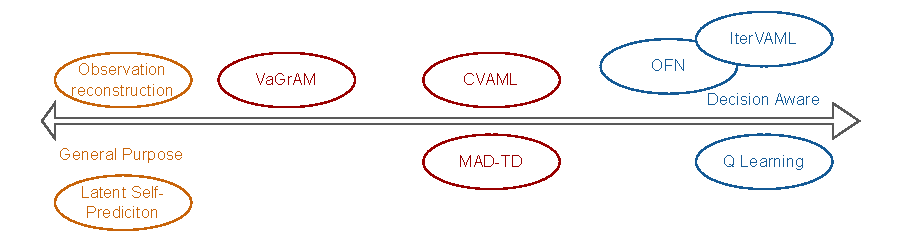
\includegraphics{illustrations/thesis_daml_spectrum.pdf}    
    \caption{A visual representation of the spectrum between decision-aware and general purpose learning.
    Several approaches presented in this thesis, such as VaGraM (\autoref{chap:vagram}), CVAML (\autoref{chap:cvaml}), and MAD-TD (\autoref{chap:mad}) combine methods from both general purpose and decision-aware learning to achieve stable and efficient \ac{rl}.
    OFN (\autoref{chap:overestimation}) only consider model-free RL and can therefore be seen as a purely decision-aware method.
    Finally, while latent self-prediction and observation reconstruction are general purpose methods, \autoref{chap:understanding} investigates how they can be used in synergy with TD learning.
    Based on this investigation, latent self-prediction is used to obtain a strong hybrid methods such as MAD-TD.}
    \label{fig:background:spectrum}
\end{figure}

The major problem that motivates the work conducted in this thesis is that the current value function alone does not necessarily provide sufficient information to learn good representations or world models.
As discussed in the introduction, reinforcement learning is fundamentally non-stationary in nature, which means that the current prediction task is not necessarily indicative of future prediction tasks.

To understand the problem intuitively, a sparse reward setting is instructive: when the task requires exploration, the value function is driven to predict $0$ for all visited states until the agent has actually reached the goal and observed positive reward.
A model or representation can then collapse the whole state space into a single feature, as no value other than 0 needs to be predicted, and potentially completely prevent further exploration.

This phenomenon is for example partially discussed by \textcite{tomar2023learning}, who show that many techniques for value-based abstractions fail in hard-exploration scenarios.
Similarly, \textcite{kemertas2021towards} show that auxiliary training objectives strongly improve the performance of bisimulation-based representation learning, especially with sparse rewards.
A related discussion in the the context of IterVAML will be presented in \autoref{chap:vagram}.
Finally, \textcite{nikishin2022primacy} conjecture the existence of a \emph{primacy bias}, the tendency of neural network-based value functions to overfit initial experience and to lose capacity to represent information obtained later in training.
This notion of the primacy bias will be addressed in detail in \autoref{chap:overestimation} and \autoref{chap:mad}, and we will see that the primacy bias can be related to the problems of learning representations and models from purely decision-aware objectives.

However, while decision-aware methods face challenges with stability, their great advantage lies in the fact that they can adapt to the task.
While general-purpose methods are often more robust to shifts in the task and missing value information, they fail to be as efficient as the latter especially under resource constraints such as network size.
Examples of this are presented in \autoref{chap:understanding} and \autoref{chap:vagram} where we see the benefits of using decision-aware algorithms when the observation space contains irrelevant distracting dimensions.
Therefore, instead of exploring decision-awareness and general-purpose learning as opposing ideas, this thesis is instead looking to find synergy which allows us to take advantage of both paradigms.
This idea is visualized in \autoref{fig:background:spectrum}, where the approaches presented in this thesis are roughly visualized along a spectrum between general-purpose and decision-aware learning.

